\subsection{Time offset turning} \label{sec:KP_timeoffset}
\begin{figure}[htbp]
  \centering
  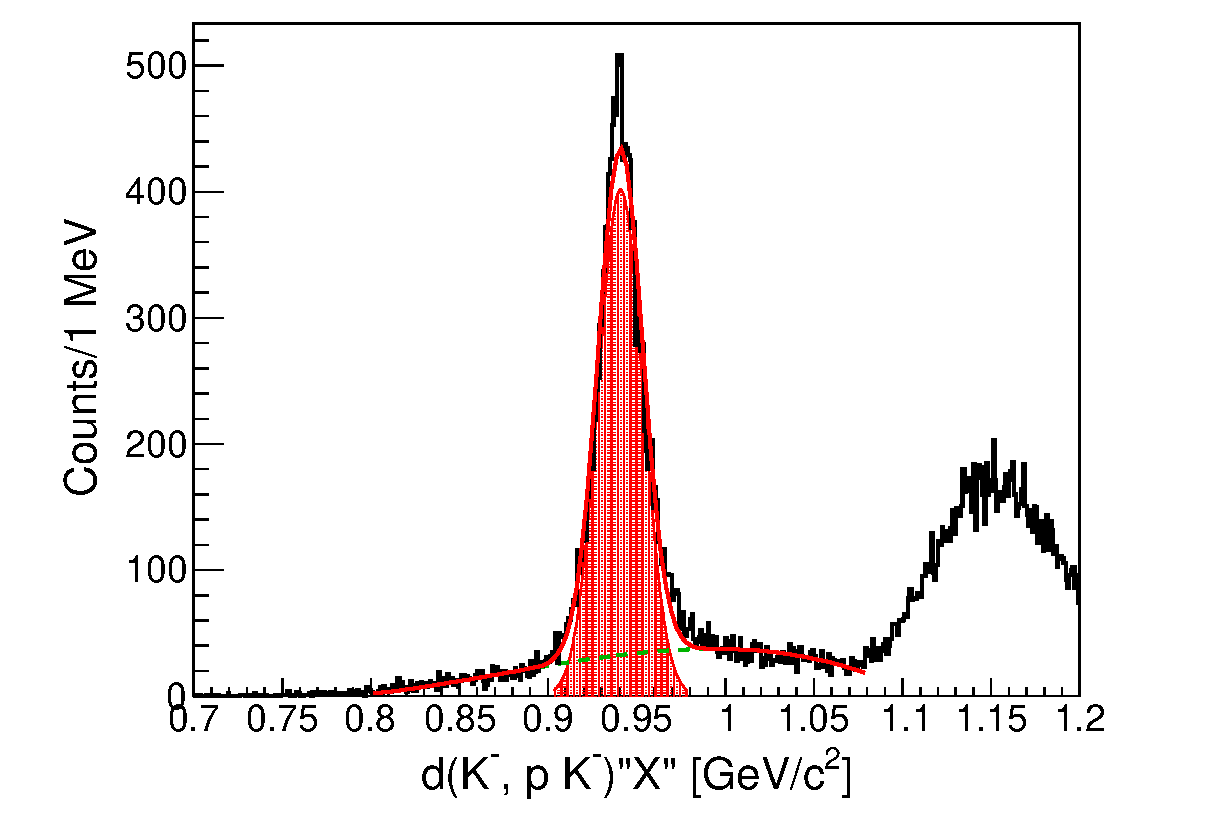
\includegraphics[width=8cm]{../pic/Run68/KP_ana/KPkm_MM.eps}
  \caption{
    This figure shows the missing mass spectrum of $d(K^-, p K^-)"X"$ in events detected the forward proton by the PC/CVC and the $K^-$ by the CDS.
    The missing neutron peak was clearly seen. 
    The fitting performed the Gaussian as peak and third polynomial function as the background.
    The red line, the red hatched region, and the broken green line indicate whole fitting line, the peak of Gaussian, and the background, respectively.
  }
  \label{fig:KPkm_MM}
\end{figure}

\begin{figure}[htbp]
  \centering
  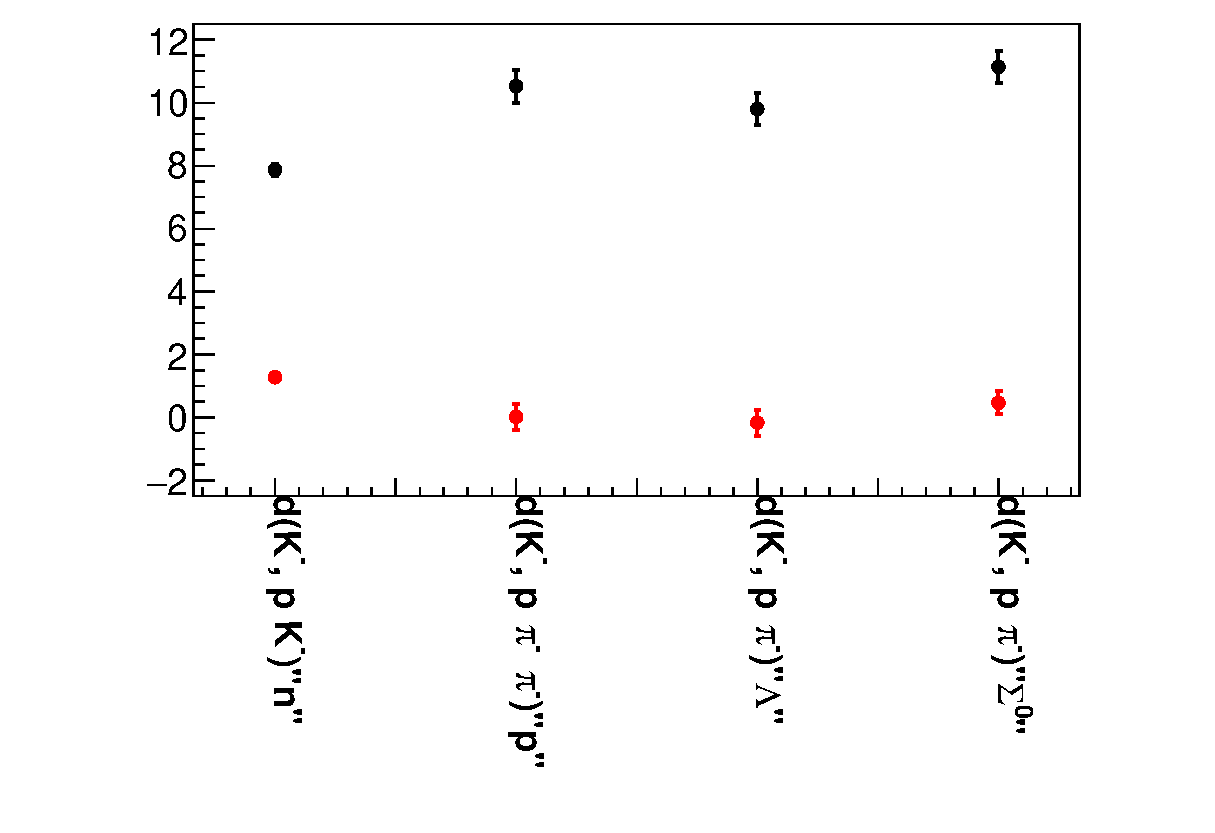
\includegraphics[width=12cm]{../pic/Dron/KP_ana/KP_diff_PDG.eps}
  \caption{
    The figure indicates differences from the PDG value of missing masses of well-known particles.
    The black plot and the red plot  indicate missing masses before and after the calibration, respectively.
  }
  \label{fig:KP_diff_PDG}
\end{figure}

Time offset was calibrated using $\pi^-$ beam through run for the segment by segment calibration.
In that run, the $\pi$ momentum used the value analyzed by the D5 magnet.

The shift of time offset that seems due to the ambiguity of the alignment was seen in the missing masses of well-known particles,
$d(K^-, p K^-)"n"$, $d(K^-, p \pi^- \pi^-)"p"$, $d(K^-, p \pi^-)"\Lambda"$ and $d(K^-, p \pi^-)"\Sigma^0"$.
The Fig\ref{fig:KPkm_MM} shows the missing mass spectrum of the $d(K^-, p K^-)"X"$ in which the missing $n$ peak is clearly seen.
The other missing mass spectra were used as signals and explained in the Sec\ref{sec:KPpimpim}.
The calibration of these time shifts was performed to become missing masses to the PDG values.
In this calibration, the beam momentum and decay particle momentum detected by the CDS was fixed and the time offset of the PC/CVC was determined to give correct masses.
As a result, these missing masses were calibrated as the Fig\ref{fig:KP_diff_PDG},
in which black plots indicate peak position before the calibration and the red plots indicate these after the calibration, respectively.
By this calibration, differences from the PDG value of these missing masses were within 2 $MeV/c^2$.


